\section{Mode-independent core architecture}
\label{sec:arch}

\subsection{The staged pipeline}

The node is a set of workers joined by blocking queues (Figure~\ref{fig:pipeline}).
The render stage, the store and the sender are the same in every mode. Only the
\code{IoStack} underneath them changes. \code{make\_io\_stack(IoMode)} builds an
\code{InboundTransport} (accept and read) and an \code{OutboundTransport} (open,
send, close). In the multiplexed modes a single object implements both halves.

\begin{figure}[h]
\centering
\begin{tikzpicture}[
    box/.style={draw, rounded corners=2pt, minimum height=8mm, minimum width=21mm,
                font=\small, align=center},
    q/.style={-{Stealth[length=2mm]}, thick},
    lbl/.style={font=\scriptsize, midway, fill=white, inner sep=1pt}]
  \node[box] (render) {Render\\\scriptsize terminal / headless};
  \node[box, right=26mm of render] (store) {StoreWorker\\\scriptsize conversations};
  \node[box, right=24mm of store] (sender) {SenderWorker\\\scriptsize write policy};
  \node[box, below=13mm of store, minimum width=40mm] (in) {InboundTransport\\\scriptsize accept, read, \code{FrameChannel}};
  \node[box, below=13mm of sender, minimum width=36mm] (out) {OutboundTransport\\\scriptsize open, send, close};
  \node[draw, dashed, rounded corners, inner sep=4pt, fit=(in)(out),
        label={[font=\scriptsize]below:IoStack, built by \code{make\_io\_stack(IoMode)}}] {};
  \draw[q] (render.20) -- node[font=\scriptsize, above, pos=0.5] {store queue} (store.160);
  \draw[q] (store.200) -- node[font=\scriptsize, below, pos=0.5] {render queue} (render.340);
  \draw[q] (store) -- node[font=\scriptsize, above] {sender queue} (sender);
  \draw[q] (in) -- node[lbl, right=2pt] {peer events, messages} (store);
  \draw[q] (sender) -- (out);
\end{tikzpicture}
\caption{The staged pipeline. Everything above the dashed box is identical in all nine modes.}
\label{fig:pipeline}
\end{figure}

\begin{itemize}
  \item \textbf{\code{StoreWorker}} is single-threaded. It owns conversations and
        subscriptions, and in benchmark (echo) mode it bounces every message back
        to its sender.
  \item \textbf{\code{SenderWorker}} owns all write policy. A transport only opens,
        writes and closes. The policy is:
        \begin{itemize}
          \item what the handshake frames contain;
          \item retries: three attempts, 100\,ms apart, with a 500\,ms
                \code{SO\_SNDTIMEO} on blocking sends;
          \item backpressure: a full transmit buffer (1\,MiB per connection) returns
                \code{WouldBlock} and the message is dropped and counted, with no
                retry or sleep;
          \item port 0 means ``never dial'';
          \item while quitting, nothing is dialled or retried.
        \end{itemize}
  \item \textbf{\code{FrameChannel}} holds the protocol state of one TCP byte stream:
        the frame decoder, the identity learned in the handshake, and forwarding to
        the store. It has no socket. Whatever owns the socket feeds it through
        \code{on\_bytes()} and reports the end through \code{on\_closed()}.
\end{itemize}

\subsection{One controller, two front ends}

\code{ChatController} contains the front-end logic: command parsing, the current
conversation, and the meaning of each store event. It does no input or output of its
own. It writes through a small \code{RenderSink} interface, which has two
implementations:
\begin{itemize}
  \item the interactive terminal UI;
  \item a headless worker that reads commands from stdin and writes one JSON object
        per line.
\end{itemize}
Commands and store events reach the headless worker through the same queue, so they
are handled in one total order. A \code{\#<req-id>} prefix on a command comes back as
\code{"re"} on its eventual reply, and \code{/sync} acts as a barrier that proves the
store has processed every earlier command. This is what makes the end-to-end tests
and the benchmark nodes deterministic.

\subsection{Identifiers and why fds are never keys}

Every id is local to the process that created it. Table~\ref{tab:ids} lists them.
The kernel reuses a file descriptor as soon as it is closed. A table keyed by fd can
therefore deliver a late event for a closed socket to whichever connection has just
been given the same number (an ABA error). Nothing above the pools uses fds:
\begin{itemize}
  \item the pools give out ids that only increase;
  \item handles are never reused, so a stale handle can only miss;
  \item in the split modes, shared ownership keeps an fd open until both pollers
        have removed it.
\end{itemize}

\begin{table}[h]
\centering\small
\begin{tabularx}{\linewidth}{@{}lXl@{}}
\toprule
Id & Purpose & Unique within \\
\midrule
peer id & this node's name for a remote peer & node, forever \\
assigned id & the remote node's name for us, re-presented on reconnect & remote node \\
\code{ChannelRef::connection\_id} & which TCP stream currently holds a peer's rx or tx slot & node, one stream \\
conversation id & one chat history & node, forever \\
handle & what the sender passes to \code{send()} and \code{close()} & one transport, never reused \\
pool id & key inside a connection pool, equal to the handle in pool modes & one pool \\
fd & the kernel descriptor, only inside \code{TcpConnection} & process, \emph{reused} \\
\bottomrule
\end{tabularx}
\caption{Identifier domains.}
\label{tab:ids}
\end{table}

\subsection{Simplex and duplex peer links}

A peer link has an \emph{rx slot} (the stream we read the peer from) and a
\emph{tx slot} (the stream we write to it). Both are stored in the \code{PeerTable}
as a \code{ChannelRef\{connection\_id, handle\}}. The wire format is the same in both
shapes; only the path of the reply differs (Figure~\ref{fig:handshake}):
\begin{itemize}
  \item In \textbf{simplex}, the acceptor dials back to the endpoint the dialler
        advertised, and sends the \code{ConnectAck} on that second connection.
  \item In \textbf{duplex}, the acceptor answers on the connection it accepted.
\end{itemize}
A simplex handshake therefore costs a TCP connect, the \code{Connect}, a second
connect and the \code{Ack}: about 3\,RTT before both sides are ready. A duplex
handshake costs about 2\,RTT.

\begin{figure}[h]
\centering
\begin{minipage}[t]{0.5\linewidth}\vspace{0pt}\centering
  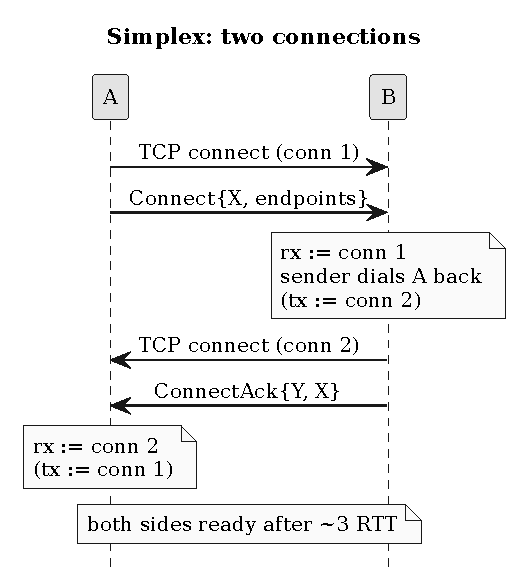
\includegraphics[scale=0.85]{handshake_simplex}
\end{minipage}%
\begin{minipage}[t]{0.5\linewidth}\vspace{0pt}\centering
  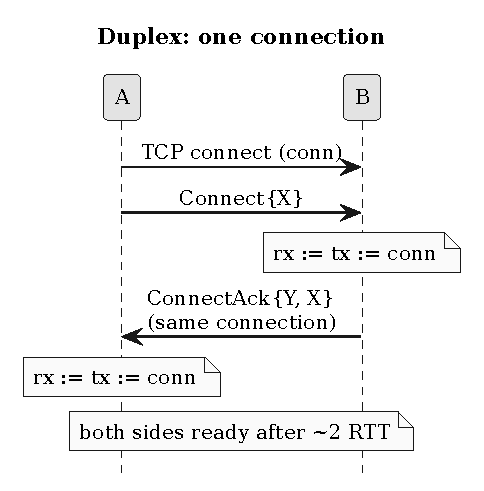
\includegraphics[scale=0.85]{handshake_duplex}
\end{minipage}
\caption{Handshake when A dials B, in the two link shapes. In simplex, A writes on
         conn~1 and B writes on conn~2.}
\label{fig:handshake}
\end{figure}

Three rules hold in both shapes:
\begin{itemize}
  \item \textbf{The newest channel wins a slot.} A release only counts if its
        \code{connection\_id} is still current, so a superseded channel closes
        silently.
  \item \textbf{Exactly one \code{EventPeerDisconnected} per peer.}
  \item \textbf{A channel that closes during its own handshake binds nothing.} A
        small lock and a \code{closing\_} flag guard both the bind and
        \code{on\_closed()}, so a \code{Connect} or \code{Ack} that arrives late on a
        closing channel attaches no slot.
\end{itemize}
The two shapes cannot interoperate: each side would wait for the reply on the wrong
socket. Every node in a run, and the load generator, must use the same shape.

\subsection{Problems met during implementation}
\label{sec:lessons}

Several problems only showed up once the nodes ran under load. Each one taught
something about the socket API or about sharing sockets between threads:
\begin{itemize}
  \item \textbf{File descriptors are reused at once.} With several threads touching
        the same sockets, any table keyed by fd can route a late event to a new
        connection that has been given the old number. The design therefore keeps fds
        inside \code{TcpConnection} and uses ids that only increase everywhere else
        (Table~\ref{tab:ids}).
  \item \textbf{Check-then-act across threads is a race.} The sender first checked
        whether a peer's tx slot was empty and then, in a separate step, decided
        whether to dial. The I/O thread could release the slot in between, and the
        sender then dialled a churned duplex peer at port~0. Such a \code{connect()}
        does not fail at once: it blocks for about 130\,s while the kernel retries the
        SYN. The node stalled in about 1 in 20 duplex runs at 50 reconnects/s. The
        decision has to be made on the same lookup that found the slot empty.
  \item \textbf{A blocking \code{connect()} on a shared thread is expensive.} The
        same blocking dial that caused the stall above is what makes the simplex
        dial-back saturate the sender over a WAN (Section~\ref{sec:res-wan}).
  \item \textbf{Shutdown is a state of the write policy.} After \code{/quit}, a
        backlog of echoes for peers that had already left kept the sender re-dialling
        them, at about 0.2\,s per message. Quitting has to stop all dialling and
        retries, not only the threads.
  \item \textbf{A connection can close during its own handshake.} A \code{Connect}
        or \code{Ack} that arrived late on a closing channel could bind a slot that
        nobody would release. The bind and \code{on\_closed()} now share a small lock
        and a \code{closing\_} flag.
  \item \textbf{Tests need real readiness, not sleeps.} Test binaries running in
        parallel collided on fixed ports, and random ports could be held by another
        process. The tests now redraw a port on a collision and wait for the
        listener's ready callback instead of sleeping.
\end{itemize}
